\documentclass{tufte-book}

% chapter format
\titleformat{\chapter}%
  {\huge\rmfamily\itshape}% format applied to label+text
  {\llap{{\parbox{1.5cm}{\hfill\itshape\huge\thechapter}}}}% label
  {2pt}% horizontal separation between label and title body
  {}% before the title body
  []% after the title body

\setcounter{secnumdepth}{2}

\hypersetup{colorlinks}
% uncomment this line if you prefer colored hyperlinks
%(e.g., for onscreen viewing)

%%
% Book metadata
\title{Field Manual: Kiiminki 3068}
\author{Tuukka Turto}
%\publisher{N/A}

%%
% If they're installed, use Bergamo and Chantilly from www.fontsite.com.
% They're clones of Bembo and Gill Sans, respectively.
%\IfFileExists{bergamo.sty}{\usepackage[osf]{bergamo}}{}% Bembo
%\IfFileExists{chantill.sty}{\usepackage{chantill}}{}% Gill Sans

%\usepackage{microtype}

%%
% Just some sample text
\usepackage{gensymb}
\usepackage{lipsum}
\usepackage{geometry}
\usepackage{amsmath}

\geometry{paper=a4paper}

%%
% For nicely typeset tabular material
\usepackage{booktabs}

%%
% For graphics / images
\usepackage{graphicx}
\setkeys{Gin}{width=\linewidth,totalheight=\textheight,keepaspectratio}
\graphicspath{{graphics/}}

% The fancyvrb package lets us customize the formatting of verbatim
% environments.  We use a slightly smaller font.
\usepackage{fancyvrb}
\fvset{fontsize=\normalsize}

%%
% Prints argument within hanging parentheses (i.e., parentheses that take
% up no horizontal space).  Useful in tabular environments.
\newcommand{\hangp}[1]{\makebox[0pt][r]{(}#1\makebox[0pt][l]{)}}

%%
% Prints an asterisk that takes up no horizontal space.
% Useful in tabular environments.
\newcommand{\hangstar}{\makebox[0pt][l]{*}}

%%
% Prints a trailing space in a smart way.
\usepackage{xspace}

% Prints the month name (e.g., January) and the year (e.g., 2008)
\newcommand{\monthyear}{%
  \ifcase\month\or January\or February\or March\or April\or May\or June\or
  July\or August\or September\or October\or November\or
  December\fi\space\number\year
}


% Prints an epigraph and speaker in sans serif, all-caps type.
\newcommand{\openepigraph}[2]{%
  %\sffamily\fontsize{14}{16}\selectfont
  \begin{fullwidth}
  \sffamily\large
  \begin{doublespace}
  \noindent\allcaps{#1}\\% epigraph
  \noindent\allcaps{#2}% author
  \end{doublespace}
  \end{fullwidth}
}

% Inserts a blank page
\newcommand{\blankpage}{\newpage\hbox{}\thispagestyle{empty}\newpage}

\usepackage{units}

% Typesets the font size, leading, and measure in the form of 10/12x26 pc.
\newcommand{\measure}[3]{#1/#2$\times$\unit[#3]{pc}}

% Macros for typesetting the documentation
\newcommand{\hlred}[1]{\textcolor{Maroon}{#1}}% prints in red
\newcommand{\hangleft}[1]{\makebox[0pt][r]{#1}}
\newcommand{\hairsp}{\hspace{1pt}}% hair space
\newcommand{\hquad}{\hskip0.5em\relax}% half quad space
\newcommand{\TODO}{\textcolor{red}{\bf TODO!}\xspace}
\newcommand{\ie}{\textit{i.\hairsp{}e.}\xspace}
\newcommand{\eg}{\textit{e.\hairsp{}g.}\xspace}
\newcommand{\na}{\quad--}% used in tables for N/A cells
\providecommand{\XeLaTeX}{X\lower.5ex\hbox{\kern-0.15em\reflectbox{E}}\kern-0.1em\LaTeX}
\newcommand{\tXeLaTeX}{\XeLaTeX\index{XeLaTeX@\protect\XeLaTeX}}
% \index{\texttt{\textbackslash xyz}@\hangleft{\texttt{\textbackslash}}\texttt{xyz}}
\newcommand{\tuftebs}{\symbol{'134}}% a backslash in tt type in OT1/T1
\newcommand{\doccmdnoindex}[2][]{\texttt{\tuftebs#2}}% command name -- adds backslash automatically (and doesn't add cmd to the index)
\newcommand{\doccmddef}[2][]{%
  \hlred{\texttt{\tuftebs#2}}\label{cmd:#2}%
  \ifthenelse{\isempty{#1}}%
    {% add the command to the index
      \index{#2 command@\protect\hangleft{\texttt{\tuftebs}}\texttt{#2}}% command name
    }%
    {% add the command and package to the index
      \index{#2 command@\protect\hangleft{\texttt{\tuftebs}}\texttt{#2} (\texttt{#1} package)}% command name
      \index{#1 package@\texttt{#1} package}\index{packages!#1@\texttt{#1}}% package name
    }%
}% command name -- adds backslash automatically
\newcommand{\doccmd}[2][]{%
  \texttt{\tuftebs#2}%
  \ifthenelse{\isempty{#1}}%
    {% add the command to the index
      \index{#2 command@\protect\hangleft{\texttt{\tuftebs}}\texttt{#2}}% command name
    }%
    {% add the command and package to the index
      \index{#2 command@\protect\hangleft{\texttt{\tuftebs}}\texttt{#2} (\texttt{#1} package)}% command name
      \index{#1 package@\texttt{#1} package}\index{packages!#1@\texttt{#1}}% package name
    }%
}% command name -- adds backslash automatically
\newcommand{\docopt}[1]{\ensuremath{\langle}\textrm{\textit{#1}}\ensuremath{\rangle}}% optional command argument
\newcommand{\docarg}[1]{\textrm{\textit{#1}}}% (required) command argument
\newenvironment{docspec}{\begin{quotation}\ttfamily\parskip0pt\parindent0pt\ignorespaces}{\end{quotation}}% command specification environment
\newcommand{\docenv}[1]{\texttt{#1}\index{#1 environment@\texttt{#1} environment}\index{environments!#1@\texttt{#1}}}% environment name
\newcommand{\docenvdef}[1]{\hlred{\texttt{#1}}\label{env:#1}\index{#1 environment@\texttt{#1} environment}\index{environments!#1@\texttt{#1}}}% environment name
\newcommand{\docpkg}[1]{\texttt{#1}\index{#1 package@\texttt{#1} package}\index{packages!#1@\texttt{#1}}}% package name
\newcommand{\doccls}[1]{\texttt{#1}}% document class name
\newcommand{\docclsopt}[1]{\texttt{#1}\index{#1 class option@\texttt{#1} class option}\index{class options!#1@\texttt{#1}}}% document class option name
\newcommand{\docclsoptdef}[1]{\hlred{\texttt{#1}}\label{clsopt:#1}\index{#1 class option@\texttt{#1} class option}\index{class options!#1@\texttt{#1}}}% document class option name defined
\newcommand{\docmsg}[2]{\bigskip\begin{fullwidth}\noindent\ttfamily#1\end{fullwidth}\medskip\par\noindent#2}
\newcommand{\docfilehook}[2]{\texttt{#1}\index{file hooks!#2}\index{#1@\texttt{#1}}}
\newcommand{\doccounter}[1]{\texttt{#1}\index{#1 counter@\texttt{#1} counter}}

\usepackage{fancybox}
\usepackage{multirow}

% Generates the index
\usepackage{makeidx}
\makeindex

\begin{document}

% Front matter
\frontmatter

% r.3 full title page
\maketitle


% v.4 copyright page
\newpage
\begin{fullwidth}
~\vfill
\thispagestyle{empty}
\setlength{\parindent}{0pt}
\setlength{\parskip}{\baselineskip}
Copyright \copyright\ \the\year\ \thanklessauthor

\par Licensed under CC BY-SA 4.0.\index{license}

\par Uniforms based on works of Tounushi (http://tounushi.deviantart.com/art/Generic-uniforms-211713655)

\par Unit insignias are from http://game-icons.net/, originally licensed under CC BY 3.0

\end{fullwidth}

% r.5 contents
\setcounter{tocdepth}{1}
\tableofcontents
\listoffigures
\listoftables

%%
% Start the main matter (normal chapters)
\mainmatter


\chapter{Kiiminki System}
\label{ch:kiiminki-system}

\newthought{Kiiminki} is a star system located at xxx-yyy.

\section{Kiiminki Star}

\newthought{Kiiminki} is a star.

\bigskip
\begin{table}
\begin{minipage}{\textwidth}
\begin{center}
\begin{tabular}{llll}
\toprule
System Name: & \multicolumn{3}{l}{Kiiminki} \\
Star Name: & \multicolumn{3}{l}{Kiiminki} \\
Star Type: & \multicolumn{3}{l}{K0V} \\
\quad Recharge Time: & \multicolumn{3}{l}{191 hours} \\
\quad Proximity Limit: & \multicolumn{3}{l}{549 564 113 km} \\
\quad Transit Time: & \multicolumn{3}{l}{5.48 days} \\

\multicolumn{4}{l}{Planets} \\
\quad 0.32 AU & J\"{a}nni      & 4.16 AU  & Keyritty \\
\quad 0.56 AU & Kakkuri    & 8.0 AU   & Meiko \\
\quad 0.8 AU  & Kuolimo    & 15.68 AU & Maintainen \\
\quad 1.28 AU & Jalanti    & 31.04 AU & Kuorinka \\
\quad 2.24 AU & Iso-Lankko & & \\

\bottomrule
\end{tabular}
\end{center}
\end{minipage}
\caption{Stellar Data of Kiiminki}
\end{table}

\section{J\"{a}nni}

\newthought{J\"{a}nni} is the first planet of Kiiminki system. Being a gas
giant near a star, J\"{a}nni is particularly hostile environment and hasn't
been explored much. Two probes have been sent onto it, but they didn't
survive for very long.

Currently J\"{a} is not of particular interest to Kingdom of Kiiminki and there
are no further scientific missions planned for it.

\bigskip
\begin{table}
\begin{minipage}{\textwidth}
\begin{center}
\begin{tabular}{ll}
\toprule
Planet Name: & J\"{a}nni \\
Planet Type: & Gas Giant \\
Position in System: & 1 \\
Orbit: & 0.32 AU \\
Moons: & 3 \\
Diameter: & 130 000 km \\
Density: & 1.2 g/cm\textsuperscript{3} \\
Surface Gravity: & 2.2 G \\
Day Length: & 13 h \\
Year Length: & 0.20 terran years \\
Habitable: & No \\
\quad Atmospheric Density: & N/A \\
\quad Atmosphere Composition: & Hydrogen, Helium \\
\quad Surface Temperature: & N/A \\
\quad Percent Surface Water: & N/A \\
\quad Highest Life Form: & N/A \\

\bottomrule
\end{tabular}
\end{center}
\end{minipage}
\caption{Planetary Data of J\"{a}nni}
\end{table}

\section{Kakkuri}

\newthought{Kakkuri} is the second planet of Kiiminki system. While the
atmosphere is not breathable, conditions on the planet are mostly tolerable.
Because of close proximity of the Kiiminki and thing atmosphere, radiation
levels can be quite high from time to time. Kakkuri seems to lack magnetic
field that would protect it from the radiation.

Surface of the Kakkuri is dotted with impact craters and ragged mountain
regions. Evidence suggests that the planet had very intense vulcanic activity
at some point during its life time, but that has ceased.

Kakkuri has some amount of mineral resources that are easily accesible and a
small mining colony by Saarinen Mining has been estabilished there.
Low gravity makes it easy to transport resources off world.

\bigskip
\begin{table}
\begin{minipage}{\textwidth}
\begin{center}
\begin{tabular}{ll}
\toprule
Planet Name: & Kakkuri \\
Planet Type: & Terrestrial \\
Position in System: & 2 \\
Orbit: & 0.56 AU \\
Moons: & 0 \\
Diameter: & 9 500 km \\
Density: & 4.18 g/cm\textsuperscript{3} \\
Surface Gravity: & 0.57 G \\
Day Length: & 18 h \\
Year Length: & 0.47 terran years \\
Habitable: & No \\
\quad Atmospheric Density: & Low \\
\quad Atmosphere Composition: & Nitrogen, Carbon Dioxide \\
\quad Surface Temperature: & 317K \\
\quad Percent Surface Water: & 0\% \\
\quad Highest Life Form: & N/A \\
\toprule
Noble Ruler: & \\
Political Ruler: & \\
HPG Class: & No service \\
Population: & 2 500 \\
USILR Code: & D-D-A-D-F \\
Notable Military Units: & \\
Major Industries: & Saarinen Mining \\
Notes: & \\


\bottomrule
\end{tabular}
\end{center}
\end{minipage}
\caption{Planetary Data of Kakkuri}
\end{table}

\section{Kuolimo}

\newthought{Kuolimo} is the third planet of Kiiminki system. It is also
called Kiiminki Prime, being the first planet settled in the system.
Kuolimo is the only planet in the system that is habitable for humans,
without special gear. The climate is cold, most of the planet is covered
in snow and ice, so some protective gear is still needed.

Kuolimo has four large continents and several clusters of islands. While
most of them are covered under ice, equatorial band is free of snow and
ice. In addition to that, areas of volcanic activity are warmer and have
less ice or are free of ice during summer months.

Climate around the equator is the most habitable, so settlements have
clustered on that area. Outposts, scientific compounds and some other
structures are located outside of the equator band, but they tend to
be rarer.

In areas that are mostly free of snow, small forests of coniferous trees grow.
Small mammals thrive in the woods, but largest species are found in the oceans
that shelter them from cold.

\marginnote{Rules for effects of snow can be found on page 60 of Tactical
Operations.}

\bigskip
\begin{table}
\begin{minipage}{\textwidth}
\begin{center}
\begin{tabular}{ll}
\toprule
Planet Name: & Kuolimo / Kiiminki Prime \\
Planet Type: & Terrestrial \\
Position in System: & 3 \\
Orbit: & 0.8 AU \\
Moons: & 0 \\
Diameter: & 12 500 km \\
Density: & 4.18 g/cm\textsuperscript{3} \\
Surface Gravity: & 0.74 G \\
Day Length: & 25 h \\
Year Length: & 0.80 terran years \\
Habitable: & Yes \\
\quad Atmospheric Density: & Normal \\
\quad Atmosphere Composition: & Nitrogen, Oxygen \\
\quad Surface Temperature: & 265K \\
\quad Percent Surface Water: & 70\% \\
\quad Highest Life Form: & Mammals \\
\toprule
Noble Ruler: & \\
Political Ruler: & \\
HPG Class: & No service \\
Population: & \\
USILR Code: & C-C-B-C-C \\
Notable Military Units: & \\
Major Industries: & \\
Notes: & \\

\bottomrule
\end{tabular}
\end{center}
\end{minipage}
\caption{Planetary Data of Kuolimo}
\end{table}

\section{Jalanti}

\newthought{Jalanti} is the fourth planet of Kiiminki system and one of
the few with settlement on it. The atmosphere of Jalanti is unbreathable
and temperature too cold for humans to survive without protective gear
or suitable vehicles. However, Jalanti has relatively rich deposits of
minerals that have attracted people to build small semi-permanent
settlement there. \marginnote{Internal combustion engines are not usable
at Jalanti, thus miners are using either fuel-cell or fusion reactor
powered vehicles.}

Jalanti Mining Station is small, mostly sub-surface, town. The exact
number of inhabitants depend on supply and demand of the minerals, but
is generally around 50 000. The mining station isn't fully
self-sufficient, but relies on materials sent from the Kiiminki Prime.

Jalanti is relatively smooth and doesn't have large mountain ranges. The
surface is dotted with impact craters like all the terrestrial type planets
without protective atmosphere. It's notable, that Jalanti has strong magnetic
field that protects it from solar wind and other forms of radiation.

\bigskip
\begin{table}
\begin{minipage}{\textwidth}
\begin{center}
\begin{tabular}{ll}
\toprule
Planet Name: & Jalanti \\
Planet Type: & Terrestrial \\
Position in System: & 4 \\
Orbit: & 1.28 AU \\
Moons: & 2 \\
Diameter: & 11 500 km \\
Density: & 6.33 g/cm\textsuperscript{3} \\
Surface Gravity: & 1.04 G \\
Day Length: & 24 h \\
Year Length: & 1.62 terran years \\
Habitable: & No \\
\quad Atmospheric Density: & Low \\
\quad Atmosphere Composition: & Ammonia \\
\quad Surface Temperature: & 210K \\
\quad Percent Surface Water: & 0\% \\
\quad Highest Life Form: & N/A \\
\toprule
Noble Ruler: & \\
Political Ruler: & \\
HPG Class: & No service \\
Population: & 50 000 \\
USILR Code: & C-C-A-D-F \\
Notable Military Units: & \\
Major Industries: & Lund Mining Consortium  \\
Notes: & \\

\bottomrule
\end{tabular}
\end{center}
\end{minipage}
\caption{Planetary Data of Jalanti}
\end{table}

\section{Iso-Lankko}

\newthought{Iso-Lankko} is the fifth planet of Kiiminki system. As it is ice
giant type of planet, it doesn't offer anything particularly interesting
except maybe for planetary scientists. Pressure and temperature at the surface
of the planet is too high for anything mechanical to survive there for long.
Thus Iso-Lankko hasn't been colonnized and only few scientific missions has
been sent to it.

\bigskip
\begin{table}
\begin{minipage}{\textwidth}
\begin{center}
\begin{tabular}{ll}
\toprule
Planet Name: & Iso-Lankko \\
Planet Type: & Ice Giant \\
Position in System: & 5 \\
Orbit: & 2.24 AU \\
Moons: & 9 \\
Diameter: & 45 000 km \\
Density: & 1.7 g/cm\textsuperscript{3} \\
Surface Gravity: & 1.09 G \\
Day Length: & 15 h \\
Year Length: & 3.76 terran years \\
Habitable: & No \\
\quad Atmospheric Density: & N/A \\
\quad Atmosphere Composition: & Methane, Ammonia \\
\quad Surface Temperature: & N/A \\
\quad Percent Surface Water: & N/A \\
\quad Highest Life Form: & N/A \\

\bottomrule
\end{tabular}
\end{center}
\end{minipage}
\caption{Planetary Data of Iso-Lankko}
\end{table}


\section{Keyritty}

\newthought{Keyritty} is the sixth planet of Kiiminki system. It is very
similar with the Iso-Lankko, as they both are ice giants. Keyritty, like
Iso-Lankko has large amount of moons that are actually more interesting than
the actual planet.

There has been plans to explore the moons more closely as they might offer a
location for setting up a remote outpost for AeroSpace forces. Such a base
would be dependent on inner system planets for the support.

\bigskip
\begin{table}
\begin{minipage}{\textwidth}
\begin{center}
\begin{tabular}{ll}
\toprule
Planet Name: & Keyritty \\
Planet Type: & Ice Giant \\
Position in System: & 6 \\
Orbit: & 4.16 AU \\
Moons: & 10 \\
Diameter: & 35 000 km \\
Density: & 1.9 g/cm\textsuperscript{3} \\
Surface Gravity: & 0.94 G \\
Day Length: & 13 h \\
Year Length: & 9.50 terran years \\
Habitable: & No \\
\quad Atmospheric Density: & N/A \\
\quad Atmosphere Composition: & Methane, Ammonia \\
\quad Surface Temperature: & N/A \\
\quad Percent Surface Water: & N/A \\
\quad Highest Life Form: & N/A \\

\bottomrule
\end{tabular}
\end{center}
\end{minipage}
\caption{Planetary Data of Keyritty}
\end{table}


\section{Meiko}

\newthought{Meiko} is the seventh planet of Kiiminki system. Meiko has a very
dense atmosphere with a extremely strong green house effect. For this reason
the surface temperature of the planet is high, even when the planet itself is
quite far away from the star.

Exploration of Meiko is problematic because of the temperature and pressure on
the surface of the planet. Thick clouds block visual instruments and only
surface radars can be used to observe the surface. There has been no
scientific missions that would have tried to land on the surface of the planet.

\bigskip
\begin{table}
\begin{minipage}{\textwidth}
\begin{center}
\begin{tabular}{ll}
\toprule
Planet Name: & Meiko \\
Planet Type: & Terrestrial \\
Position in System: & 7 \\
Orbit: & 8.0 AU \\
Moons: & 4 \\
Diameter: & 14 500 km \\
Density: & 4.78 g/cm\textsuperscript{3} \\
Surface Gravity: & 0.98 G \\
Day Length: & 22 h \\
Year Length: & 25.34 terran years \\
Habitable: & No \\
\quad Atmospheric Density: & Very High \\
\quad Atmosphere Composition: & Carbon Dioxide, Nitrogen \\
\quad Surface Temperature: & 537K \\
\quad Percent Surface Water: & 0\% \\
\quad Highest Life Form: & N/A \\

\bottomrule
\end{tabular}
\end{center}
\end{minipage}
\caption{Planetary Data of Meiko}
\end{table}

\section{Maintainen}

\newthought{Maintainen} is the eigth planet of Kiiminki system. As a large gas
giant, it poses lot of problems for exploring the surface of the planet. The
moons around it are easier objects and the largest one of them has permanent
AeroSpace base with a small detatchment of fighters of the 4th Winged
Vengeance.

AeroSpace base at moon Tupas is also where new pilots will earn their wings.
Upper atmosphere of Maintainen is a spectacular proving ground for pilots and
offer plenty of space for manoeuvres.

\bigskip
\begin{table}
\begin{minipage}{\textwidth}
\begin{center}
\begin{tabular}{ll}
\toprule
Planet Name: & Maintainen \\
Planet Type: & Gas Giant \\
Position in System: & 8 \\
Orbit: & 15.68 AU \\
Moons: & 16 \\
Diameter: & 70 000 km \\
Density: & 1.00 g/cm\textsuperscript{3} \\
Surface Gravity: & 1.00 G \\
Day Length: & 12 h \\
Year Length: & 69.55 terran years \\
Habitable: & No \\
\quad Atmospheric Density: & N/A \\
\quad Atmosphere Composition: & Hydrogen, Helium \\
\quad Surface Temperature: & N/A \\
\quad Percent Surface Water: & N/A \\
\quad Highest Life Form: & N/A \\
\toprule
Noble Ruler: & \\
Political Ruler: & \\
HPG Class: & No service \\
Population: & 1 000 \\
USILR Code: & C-F-F-F-F \\
Notable Military Units: & 4th Winged Vengeance \\
Major Industries: & \\
Notes: & Only moon Tupas has settlement \\


\bottomrule
\end{tabular}
\end{center}
\end{minipage}
\caption{Planetary Data of Maintainen}
\end{table}


\section{Kuorinka}

\newthought{Kuorinka} is the ninth planet of Kiiminki system. It consists
mostly of ice and dust. Kuorinka is a little of interest for people of
Kiiminki system. At one time there were plans to set up a remote research
station there, but the plans never materialized. Kuorinka is inhospitable
place that does not offer any natural resources to exploited.

Few exploration missions have been sent to Kuorinka and all have failed
to produce information that could be directly beneficial to the people 
of Kiiminki system. Scientifically Kuorinka is interesting, because it
is so far from the center of the star system and temperature is rather
low.

\bigskip
\begin{table}
\begin{minipage}{\textwidth}
\begin{center}
\begin{tabular}{ll}
\toprule
Planet Name: & Kuorinka \\
Planet Type: & Dwarf Terrestrial \\
Position in System: & 9 \\
Orbit: & 31.04 AU \\
Moons: & 0 \\
Diameter: & 1 800 km \\
Density: & 1.00 g/cm\textsuperscript{3} \\
Surface Gravity: & 0.03 G \\
Day Length: & 24 h \\
Year Length: & 193.70 terran years \\
Habitable: & No \\
\quad Atmospheric Density: & Vacuum \\
\quad Atmosphere Composition: & N/A \\
\quad Surface Temperature: & 42K \\
\quad Percent Surface Water: & 0\% \\
\quad Highest Life Form: & N/A \\

\bottomrule
\end{tabular}
\end{center}
\end{minipage}
\caption{Planetary Data of Kuorinka}
\end{table}


\chapter{Fifty Words for Snow}

\newthought{People of Kiiminki system} had fifty words for snow and
J\o rdis hated each and every of them with burning passion. He hated
\emph{polanne}, solidified and partly frozen snow. He hated \emph{viti}, 
freshly snowed light snow. And especially he hated \emph{kinos}, snow 
that strong wind had pushed into dune shapes. In short, J\o rdis hated 
snow in general. The problem was, that in Kiiminki prime, snow was 
everywhere.

J\o rdis sighed and continued inspecting the Snow Moose, a huge
tracked transport that had been specifically designed for arctic
environment. If there was something that he hated more than snow, it
was having his vehicle to break down in the middle of nowhere, with
nothing else than snow around him.

Snow Moose was parked in a large hall with few other vehicles.
Floodlights provided light and he had turned vehicle's work lights on
too. Hall was almost warm, just a tad below freezing temperature.
There was no point letting snowy vehicles to warm so much that the
snow would melt and start rusting the steel. J\o rdis rubbed his hands
together briefly to warm them up and continued with the inspection.
Soon he would be done and hopefully Pettersson would be there to
join the ride to the outpost where they were to deliver some
supplies.

\newthought{Diesel engine} started to rumble as J\o rdis started the
engine and performed the final check up before unhooking the heating
cables and closing the engine hatch. Pettersson was late, but that was
nothing new. J\o rdis let the engine idle and listened to the sound.
Then he saw Pettersson finally enter from the side door and wave him
before starting to open the big double doors. Finally, they were about
to start their supply run to outpost 15.

J\o rdis turned on the headlights and slowly drove the Snow Moose out
into the darkness. It was early morning and the temperature was frisky
-25\celsius. J\o rdis dreamed of living on a sandy desert planet with
twin suns, as he waited for Pettersson to close the doors behind him 
and climb into the cabin. It was time to start the supply run.

\chapter{History}
\label{ch:history}

\newthought{Kingdom of Kiiminki} was founded in 2525 when Susanna Lohtander
lead a group of settler to a new star system near Gum Nebula. Kiiminki system
wasn't particularly hospitable, but one of the planets had potable water,
which was reason enough to try colonnize it. Settlers estabilished the first
city, Laamanko, near equator where the climate was the warmest and visible 
ground meant that excavating for minerals was easy. From the original
settlement the people of Kiiminki slowly spread further on the planet, first
along the equatorial band and then later towards the poles.

Kiiminki was aiming for independence from the beginning. Being located far
away from Terra meant that communications were slow. Although Kiiminki did
posses decent natural resources, Terra was mostly not interested in it as
there were other planets with similar resources that were closer to Terra.
Thus, Kiiminki was mostly left alone as long as they nominally stayed under
the rule of Terra.

When Reunification War broke out in 2577, focus of Terra turned towards the
major periphery worlds. Kiiminki wasn't one of them, being a single star
system with only few colonnized planets. Again they were left alone and
mostly forgotten.

After the end of Reunification War, inhabitants of Kiiminki started seriously
considering their position with Terra and wars that had ravaged humankind. As
a result, Kiiminki declared independency in 2602. Their declaration was met
with modest opposition, but since the system wasn't particularly interesting,
Kiiminki was allowed independence.

\newthought{For the next 100 years} Kiiminki prospered. The system was slowly
settled and political ties with neighbouring domains were forged. When
Succession Wars broke out, Kiiminki deliberately cut ties with most of its
neighbours and decided to try to survive on it own. While this meant that
standards of living were reduced, leaders of Kiiminki felt it was better
option than risking getting drawn into war.

The decision seemed to work relatively well. Kiiminki had to defend its
borders several times, but large scale war was avoided in the end. Survival
in hostile system proved to be difficult and lot of resources had to be
directed in growing enough food and manufacturing the most basic necessities.
Trade suffered too and as a result many luxury or high-tech items were not
available anymore. Kiiminki maintained some trade with its neighbours, but
mostly it was trying to survive on its own.

Pirate forces started to be a large problem at this stage. There had always
been pirate bases nearby, but now the pirates were getting bolder and
even attacking merchant fleets in Kiiminki system. This prompted for
increased patrols by both navy and AeroSpace force. More AeroSpace assets were
acquired via trade to improve defence of the system and the merchant fleet.

\newthought{In 3050 things changed again} as the clans returned from their
exodus. While Kiiminki wasn't directly threatened, the general unrest of
Inner Sphere was visible even in their borders. Pirate activity increased even
more and AeroSpace fleet of Kiiminki had hands full trying to defend the
small nation. During this period, Kiiminki Armed Forces ventured outside of
the domain's borders several times in order to hunt down pirates and destroy
their bases. Campaign was moderately succesful, although pirate presence was
never completely eradicated.

\chapter{Sociopolitical Structure}
\label{ch:sociopolitical-structure}

\newthought{Goverment Structure}

\newthought{Monarch}

\newthought{Riksdagen}

\chapter{Cultural Structure}
\label{ch:cultural-structure}

\newthought{Religion}

\newthought{Education}

\newthought{Arts}

\chapter{Industry}
\label{ch:industry}

\newthought{Harsh conditions} of Kiiminki Prime place some limits on the
industry, but still the system has managed to develop even some high tech
industry. Mostly local industries are focused on petrochemicals, mining and
ore processing.

\newthought{Saphire Petrochemicals} is largest local petrochemical companies.
They do everything from prospecting, drilling and oil processing to more
sophisticated lines like plastics and synthetic products. The company exports
some of its products to other systems, but majority stays in the Kiiminki.

Internal combustion engines are still commonly used in Kiiminki Prime as
more sophisticated ones are too expensive and difficult to produce in large
enough quantities. Saphire Petrochemicals is refining the majority of diesel
that is being used by those engines.

\newthought{Wilkman Metal Works} is the major heavy machinery supplier. They
produce everything from railroad tracks to tanks. Wilkman Metal Works employs
a large network of subcontractors and suppliers.

Because the company is a key supplier to military, the goverment likes to
keep a close watch to it. Part of the shares of the Wilkman Metal Works is
owned by the goverment and there is a goverment representative in the board
of the company. The current representative is \O ydis Swenhaugen. Swenhaugen
has stated that her primary goal is to ensure the longevity of the company
and profits are only secondary concern.

The company has been owned by the same family since the beginning and it's
currently chaired by Olof Wilkman. As Olof Wilkman is rather old, he is soon
expected to retire from the board and hand down the duties to the next
generation of Wilkmans. Complete bio of Olof Wilkman is presented in section
\ref{sc:bio-olof-wilkman}.

\newthought{$\Delta$$\Sigma$  Motors} is the major internal combustion engine
designer and manufacturer. They products range from small and simple engines
used in consumer products to powerful military grade gas turbines used in
combat vehicles. Large portion of income for $\Delta$$\Sigma$  Motors comes
from subcontracting works for Wilkman Metal Works. Some memebers of the board
criticize this and would rather see a larger range of products, so that the
company wouldn't be so dependent on Wilkman Metal Works.

\newthought{Lund Mining Consortium} is group of smaller mining companies that
pooled their resources together in order to be able to mine some of the
more difficult deposits. The consortium is the major player in extracting and
refining minerals in areas that are covered by ice around the year.

The consortium has recently opened three new mining operations at the far
arctic. Mines have had all kinds of problems since the beginning because of
the harsh conditions, but the first one is already starting to produce ore.
The consortium expects other two mines to be in working order in no time.

The consortium exploys its own security forces that are stationed near mines
and are armed. Mostly it is just infantry, with some lightly armoured
vehicles. The more estabilished the mine is, the better it's protected.

\newthought{Saarinen Mining} is the largest mining company that is not part of
Lund Mining Consortium. It is large enough to survive without the help of the
consortium and the competition between Saarinen Mining and Lund Mining
Consortium is fierce. Both seek to claim new operations and provide much
needed ore and refined metals to Kingdom of Kiiminki.

Saarinen Mining has accused Lund Mining Consortium for fixing prices multiple
times. Lund Mining Consortium on the other hand has pointed out many safety
violations on Saarinen Mining's operations. It seems that both are ready to
quite drastic measures in order to gain advantage on market.

Saarinen Mining is currently lead by William Saarinen, who owns majority of
the shares. During period of William Saarinen, Saarinen Mining has opened new
mines in Kakkuri. The operation is still new, but so far looks very promising.

\newthought{TopTech} is largest of the companies focusing on consumer
electronics and high tech products. Main revenues come from consumer
electronics and the company doesn't currently export anythign to other
systems. TopTech is co-operating with the military in their research
programs.

As TopTech manufactures anything from toasters and microwaves to computer
chips and radars, it is hard to find a household in Kiiminki Prime that
wouldn't have any of their products. The company doesn't have monopoly in any
of its fields, but it still has a very large influence. There has been
complaints of unfair competition, but no actions have been taken so far.

\newthought{SimLine Electronics} concentrates completely on luxury electronics
for consumers. SimLine manufactures various entertainment systems and high
quality lighting systems. It has gained a small, but dedicated following from
wealthy and those wanting to appear wealthy consumers. SimLine is trying to
expand to middle wealth category, but competition with TopTech is proving to
be quite difficult.

\chapter{Military}
\label{ch:military}

\newthought{Military of Kiiminki} has always had to cope with the fact
that the system isn't not a industrial power house. They strive to
independence as much as possible, but the fact is that the military
is dependent on other systems for units and spare parts. Especially
BattleMechs can't be manufactured in the Kiiminki system.

\section{Organisation}
\label{sc:organisation}

\newthought{Military organisation} at Kiiminki Armed Forces (KAF) follow
to those of Star League to a certain degree. Commanders place a high
importance on self-reliance and independence of the fielded units.
Combined arms is favoured over single specific unit type.

\newthought{Divisions} are assembled as needed and their force
composition is tailored for the specific task in hand. However, some
standard force composition exists, that are often used as the base of
more specific force.

\bigskip
\begin{table}
\begin{minipage}{\textwidth}
\begin{center}
\begin{tabular}{ll}
\toprule
Division Type & Composition \\
\midrule
\multirow{2}{*}[0.75em]{BattleMech}          & 2 BattleMech Regiments \\ 
                                           & 1 Mechanised Infantry Regiment \\
\multirow{2}{*}[0.75em]{Armor Division}      & 2 Armor Regiments \\
                                           & 1 Mechanised Infantry Regiment \\
\multirow{2}{*}[0.75em]{Mechanised Infantry} & 3 Mechanised Infantry Regiments \\
                                           & 1 BattleMech company \\
\multirow{2}{*}[0.75em]{Infantry}            & 3 Infantry Regiments \\
                                           & 1 armor company \\
\bottomrule
\end{tabular}
\end{center}
\end{minipage}
\caption{Standard Division Organisation}
\end{table}

\newthought{BattleMechs} are hard to obtain and maintain, so they are
rarely fielded in big numbers. Usually they are tasked to serve as a
strike force, while receiving support from armors and mechanised
infantry. BattleMechs are used to strike through the enemy lines and
mechanised infantry with the help of armors exploit the opening.

\bigskip
\begin{table}
\begin{minipage}{\textwidth}
\begin{center}
\begin{tabular}{lll}
\toprule
Unit & Component Units & Total Strength \\
\midrule
Lance     & -            & 4 BattleMechs \\
Company   & 3 Lances     & 12 BattleMechs \\
Battalion & 3 Companies  & 36 BattleMechs \\
Regiment  & 3 Battalions & 108 BattleMechs \\
\bottomrule
\end{tabular}
\end{center}
\end{minipage}
\caption{Standard BattleMech Organisation}
\end{table}

\newthought{AeroSpace units} are sort of an exception in the KAF. 
\marginnote{Maintainen has long been a proving ground for AeroSpace
pilots and the place to earn pilot wings.}
They rarely get fielded in big numbers, except when no other unit can
fulfill the mission. Most often AeroSpace units are used to provide air
cover, obtain air supremacy and conduct recon and strike missions. They
are the surgical knife that a skilled commander uses to carve the battle
theater to his liking.

\bigskip
\begin{table}
\begin{minipage}{\textwidth}
\begin{center}
\begin{tabular}{lll}
\toprule
Unit & Component Units & Total Strength \\
\midrule
Lance    & -           & 2 AeroSpace Fighters \\
Squadron & 3 Lances    & 6 AeroSpace Fighters \\
Company  & 3 Squadrons & 18 AeroSpace Fighters \\
Wing     & 3 Companies & 54 AeroSpace Fighters \\
Regiment & 3 Wing      & 108 AeroSpace Fighters \\
\bottomrule
\end{tabular}
\end{center}
\end{minipage}
\caption{Standard AeroSpace Organisation}
\end{table}

\newthought{Armor forces} are the bread and butter of KAF. 
\marginnote{There is a long standing tradition that at least two armor
companies are conducting arctic training at any given time. These
assignments usually last few months, during which the unit is operating
in the arctic region of Kiiminki Prime.}
They are used for everything from scouting to strike missions and recon 
with force. Arctic conditions of Kiiminki require specialized vehicles 
and crews that understand how to fight in the freezing coldness.

Armored units are able to operate in conditions that would be too cold
for regular infantry. They are not hampered by snow storms in the same
way as AeroSpace assets are. BattleMechs are even more versatile than
armor units, but much more expensive and rarer.

\bigskip
\begin{table}
\begin{minipage}{\textwidth}
\begin{center}
\begin{tabular}{lll}
\toprule
Unit & Component Units & Total Strength \\
\midrule
Lance     & -            & 4 Vehicles \\
Company   & 3 Lances     & 12 Vehicles \\
Battalion & 3 Companies  & 36 Vehicles \\
Regiment  & 3 Battalions & 108 Vehicles \\
\bottomrule
\end{tabular}
\end{center}
\end{minipage}
\caption{Standard Armor Organisation}
\end{table}

\newthought{Mechanized and regular infantry} both use similar force
compositions. The main difference is that the mechanized infantry has
armoured personnel carriers and infantry fighting vehicles at their
disposal at all times. Use of regular infantry tends to concentrate on
defending cities and other structures, albeit some special units can be
used in offensive purposes too.
\marginnote{Arctic Foxes is foot infantry battalion that has specialized in
fighting in arctic environment without direct support. They are masters
of survival and considered as one of the elite forces of the KAF.}

Mechanized infantry is able to move quicker than the regular infantry
and their vehicles also provide cover from the elements. Close
co-operation with armor units is often trained.

\bigskip
\begin{table}
\begin{minipage}{\textwidth}
\begin{center}
\begin{tabular}{lll}
\toprule
\multicolumn{3}{l}{Standard Infantry Organisation} \\
\midrule
Unit & Component Units & Total Strength \\
\midrule
Squad     & -            & 10 Troops \\
Platoon   & 3            & 30 Troops \\
Company   & 4 Platoons   & 120 Troops \\
Battalion & 4 Companies  & 480 Troops \\
Regiment  & 4 Battalions & 1920 Troops \\
\bottomrule
\end{tabular}
\end{center}
\end{minipage}
\caption{Standard Infantry Organisation}
\end{table}

\section{Military Branches}
\label{sc:military_branches}

\newthought{Kiiminki Armed Forces} have several branches, each with their own
specilized task and mission. Each branch is lead by General.

\newthought{Army} is the boots on the ground. It consists mainly of infantry,
armor and artillery. Some of the units have organic AeroSpace component
attached to them, but army otherwise does not have any major AeroSpace
capability.

Army is currently lead by General xx yy.

\newthought{'Mech Force} mainly consists of BattleMechs, but IndustrialMechs
are used in certain support roles too. In addition to that, 'Mech Force has
some amount of mechanized infantry in them. 'Mech Force is one of the most
versatile branches and are capable of operating in very varied environments.

'Mech Force is currently lead by General xx yy.

\newthought{AeroSpace Force} operate on and around the planets with AeroSpace
fighters. It primarily conducts AeroSpace warfare, but is also responsible for
patrolling and maintaining control in inner Kiiminki system.

AeroSpace Force is currently lead by General xx yy.

\newthought{Navy} operates in deep space with warships, dropships and
jumpships. Navy performs patrol in the outer Kiiminki system and is tasked
transporting other branches from planet to planet or from system to system
when needed.

Navy works in close cooperation with the merchant fleet and collects
intelligence from them. In return, navy can provide escort for high profile
or otherwise important missions of merchant fleet.

Navy is currently lead by General xx yy.

\newthought{Intelligence} continuously gathers data from various sources,
analyzes it and provides summaries and reports when needed. While other
branches may employ recon forces on a tactical scale, intelligence has much
broader scope.

Intelligence is currently lead by General xx yy.

\newthought{Medical Corps} provides medical care to other branches. It trains
medics, nurses, doctors and other medical personnel. In addition to that,
Medical Corps performs research and development in medical field.

Combat medics of other branches are trained by Medical Corps and they may
return for additional training from time to time.

Medical Corps is currently lead by General xx yy.

\section{Military Ranks}
\label{sc:military_ranks}

\newthought{All branches of KAF} are using the same rank system.

\newthought{Private} is the lowest enlisted rank.

\newthought{Corporal} is the lowest NCO rank. Well performing private may be
promoted to this rank. Infantry squads are often lead by corporal or sergeant.
In other forces corporals may lead teams that are charged with a specific
task like maintenance or guard duty.

Specialists are often corporals. For example infantry recon squads consist
of corporals lead by sergeant major. IndustrialMech pilots in 'Mech Force
usually start as corporals.

\begin{marginfigure}[0\baselineskip]
  
\includegraphics[width=5.0cm]{rank-corporal}
  \caption{Insignia of Infantry Corporal}
  \label{fig:insignia_corporal}
\end{marginfigure}

\newthought{Sergeant} is the second NCO rank. Sergeants often lead infantry
squads. In many forces they are the backbone of the army as they keep their
unit in working order and liason between officers and non-officers.

There are substantial number of career sergeants, who have been working in
KAF for a long time, but don't have aspiration to rise to officer rank. These
sergeants are officially senior sergeants, but are adressed simply as
sergeant.

\begin{marginfigure}[0\baselineskip]
  
\includegraphics[width=5.0cm]{rank-sergeant}
  \caption{Insignia of Armor Sergeant}
  \label{fig:insignia_sergeant}
\end{marginfigure}

\newthought{Sergeant Major} is the highest NCO rank. Pilots of various kinds
are usually promoted to this rank. Sergeant majors can also lead teams or
squads of specialists.

In training units, sergeant majors often work as assistants for trainers.
They superwise and evaluate the trainees.

\begin{marginfigure}[0\baselineskip]
  
\includegraphics[width=5.0cm]{rank-sergeant-major}
  \caption{Insignia of Armor Sergeant Major from Artillery Battalion}
  \label{fig:insignia_sergeant_major}
\end{marginfigure}

\newthought{Lieutenant} is the lowest officer rank. Lieutenants, like all
officers, undergo extra leadership training in addition to the regular
training given by the military branch.

In infantry lieutenants often lead platoons or act as trainers in training
units. Being the most junior officer rank, it is well possible that a
new lieutenant is leading NCO who is older than him.

Tank commanders in army are usually lieutenants, while rest of the crew
consists of NCOs.

In 'Mech and AeroSpace forces, lieutenant is often charged of leading a
lance.

\begin{marginfigure}[0\baselineskip]
  
\includegraphics[width=5.0cm]{rank-lieutenant}
  \caption{Insignia of AeroSpace Lieutenant}
  \label{fig:insignia_lieutenant}
\end{marginfigure}

\newthought{Captains} are often found leading companies, lances or squadrons
in combat units. They can also be found in various administrative positions or
positions requiring high specialization. For example, most of the doctors
trained by the medical corps are surgeon captains or higher, regardless if
they actually can perform surgeries or not.

In combat units captain is usually the highest rank to see a direct combat.
Current doctrine places high emphasis on dynamic leadership and taking
initiative. Thus captains of combat units tend to be relatively young and
physically fit.

\begin{marginfigure}[0\baselineskip]
  
\includegraphics[width=5.0cm]{rank-captain}
  \caption{Insignia of 'Mech Captain}
  \label{fig:insignia_captain}
\end{marginfigure}

\newthought{Majors} lead battalions and wings and normally don't engage in
combat. In 'Mech Force they may still lead from the front, but only if
dual-cockpit or similar system is available. Leading whole battalion simply
doesn't leave them enough time to perform active battle duties.

Majors are also found in various administrative positions. Combat school
headmasters are usually majors or lieutenant colonels. Research projects
can be lead by majors.

\begin{marginfigure}[0\baselineskip]
  
\includegraphics[width=5.0cm]{rank-major}
  \caption{Insignia of Infantry Major}
  \label{fig:insignia_major}
\end{marginfigure}

\newthought{Lieutenant Colonel}

\begin{marginfigure}[0\baselineskip]
  
\includegraphics[width=5.0cm]{rank-lieutenant-colonel}
  \caption{Insignia of Armor Lieutenant Colonel}
  \label{fig:insignia_lieutenant_colonel}
\end{marginfigure}

\newthought{Colonel}

\newthought{Colonels} are regimental leaders. They lead and oversee training
and operation of an regiment.

Some of larger research and development programs are lead by colonels. They
usually don't get involved with single research projects, unless for auditing
or benchmarking reasons.

\begin{marginfigure}[0\baselineskip]
  
\includegraphics[width=5.0cm]{rank-colonel}
  \caption{Insignia of Navy Colonel}
  \label{fig:insignia_colonel}
\end{marginfigure}

\newthought{Brigadier Generals} are often leading divisions or in some high 
rofile administrative positions like heading a specific research complex.
All generals have same coloured insignia that does not denote a specific
branch or unit.

\begin{marginfigure}[0\baselineskip]
  
\includegraphics[width=5.0cm]{rank-brigadier-general}
  \caption{Insignia of Brigadier General}
  \label{fig:insignia_brigadier_general}
\end{marginfigure}

\newthought{Major General}

Major generals lead field armies if one has been mobilized. During the peace
time they focus on administrative duties and research. Major generals are
often responsible on overseeing development of new combat doctrine or
improvement of old one.

\begin{marginfigure}[0\baselineskip]
  
\includegraphics[width=5.0cm]{rank-major-general}
  \caption{Insignia of Major General}
  \label{fig:insignia_major_general}
\end{marginfigure}

\newthought{General}

Generals are in charge of military branches. They are responsible on overall
doctrine, training and readyness of their branch. They are often referred with
their military branch, for example infantry general or armor general.

\begin{marginfigure}[0\baselineskip]
  
\includegraphics[width=5.0cm]{rank-general}
  \caption{Insignia of General}
  \label{fig:insignia_general}
\end{marginfigure}

\newthought{Field Marshal} \marginnote{As a sign of their rank, field marshal
carries a ceremonial baton with them.} is highest rank in KAF and there
usually are only one, if any at all, person holding this rank. Field marshal
is commander of the entiner KAF force.

\section{Military Uniforms}
\label{sc:military_uniforms}

\newthought{Different branches} of KAF have adopted their own style of
uniforms that differ in style and coloring.

\begin{marginfigure}[0\baselineskip]
  
\includegraphics[width=2.5cm]{army_service}
  \caption{Standard army service uniform}
  \label{fig:army_service}
\end{marginfigure}

\newthought{Standard army service uniform} is worn by personnel of all army
units that don't have their own distinctive uniform. It consists of a coat,
shirt and trousers. Headgear for enlisted personnel is green beret and
a peaked cap for officers. In cold weather, beret and peaked cap are
substituted with a winter hat. In addition to replacing the beret with 
the winter hat, a great coat can be worn over the standard coat.

Location of rank insignia depends on whether a great coat is being worn or
not. With regular coat, rank insignia is placed on coat lapel. Exact colors
of the insignia depend on the unit. With great coat the rank insignia is
placed on sleeves, right above cuffs. Background of insignia is the same color
as the coat and rank is denoted with golden color.

The 1st Arctic Foxes wear white beret instead of the standard green one. Their
service uniform is otherwise identical with the standard army one. Both
officers and enlisted personnel wear beret with the service uniform.

Armor units, namely the 8th Tracked Death and 10th Lucky Ones wear black beret
instead of the standard green one. Their service uniform is otherwise
identical with the standard army one. Both officers and enlisted personnel
wear beret with the service uniform.

\begin{marginfigure}[0\baselineskip]
  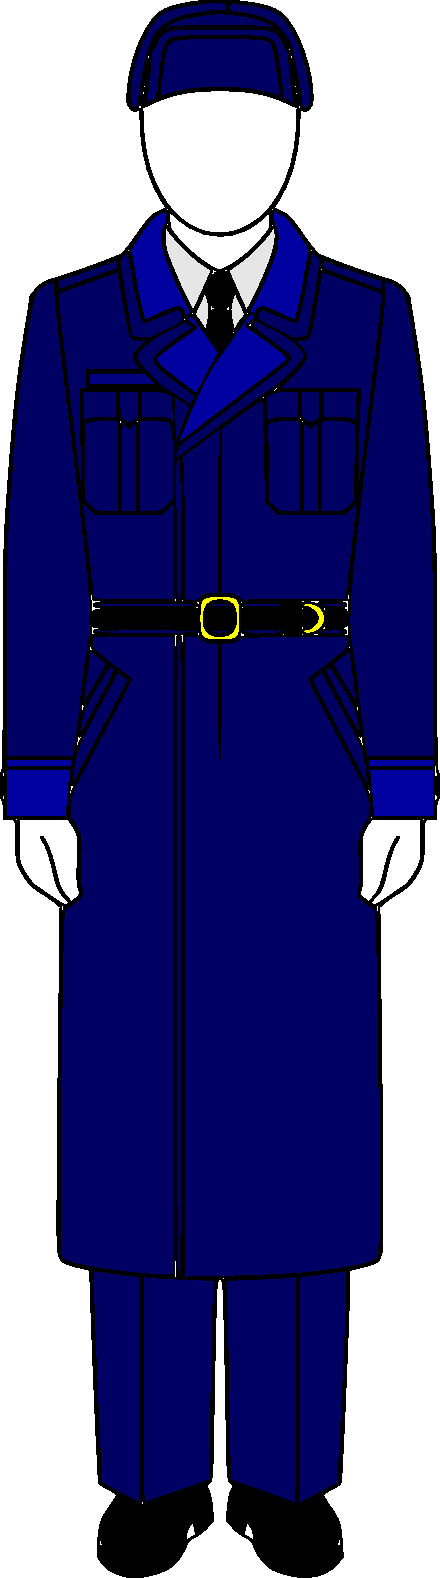
\includegraphics[width=2.5cm]{aerospace_great_coat}
  \caption{Standard AeroSpace service uniform with great coat and winter hat}
  \label{fig:aerospace_great_coat}
\end{marginfigure}

\newthought{Standard AeroSpace service uniform} is worn by personnel of all
AeroSpace units that don't have their own distinctive uniform. It consists of
a coat, shirt and trousers. Headgear for enlisted personnel is blue cap and
a peaked cap for officers. In cold weather, both caps are substituted with
a winter hat. In addition to replacing cap with the winter hat, a great coat
can be worn over the standard coat. Cut of uniform is the same with army
uniform, only the color differs.

Location of rank insignia depends on whether a great coat is being worn or
not. With regular coat, rank insignia is placed on coat lapel. Exact colors
of the insignia depend on the unit. With great coat the rank insignia is
placed on sleeves, right above cuffs. Background of insignia is the same color
as the coat and rank is denoted with golden color.

\section{Military Schools}
\label{sc:military_schools}

\newthought{Training in KAF} is done in two distinct ways. Initial training and
specialization training is done in various military schools. Further training
and fine honing of the skills is done in respective combat units. This has the
advantage that all of the units have the same basic foundation set of skills,
which makes co-operation between units easier. At the same time, there is
enough room for individual units to specialize to their respective areas.

Regardless of service branch, each individual warrior undergoes same basic
training that teaches them basics of military life and some rudimentary
infantry combat skills. This way, even dropship maintenance teams can defend
themselves in case they ever find themselves in a combat with an opposing
force.

\newthought{Oort Infantry School} is located in the equator region of Kuolimo.
It is the place where a fresh recruit takes their first steps into military
life. Basic combat courses are held here and virtually every member in KAF
has started their career here.

In addition to basic combat course, some infantry specialization courses are
held in the infantry school. These include courses for mechanized infantry,
combat engineers and anti-armor infantry.

Headmaster of Oort Infantry School is Lieutenant Colonel x x,
who has been in the post for the last 15 years.

\newthought{Kuiper Sniper School} is one of the smallest combat schools in KAF.
This is where snipers are trained for all military branches. Prospective
snipers are taught very extensive sharp shooting skills. On top of that, they
are trained in staying hidden, moving unnoticed and battlefield observation
skills.

Snipers are often used as forward observers for calling in artillery or air
strikes. For this reason they are trained to operate with signaling and
communications equipment.

Headmaster of Kuiper Sniper School is Major y y.

\newthought{Penrose Armor Academy} is the main school responsible of training
armored units for KAF.

Headmaster of Penrose Armor Academy is Major z z.

\chapter{Active Units}
\label{ch:active_units}

\section{1st Arctic Strikers}
\label{sc:arctic_strikers}

\begin{marginfigure}[0\baselineskip]
  
\includegraphics[width=3cm]{triple-yin}
  \caption{The insignia of 1st Arctic Strikers}
  \label{fig:arctic_strikers}
\end{marginfigure}

\newthought{1st Arctic Strikers} is a venerated elite unit. Members of the unit
are selected with a rigorous testing program and are serving provisionally.
If their performance or attitude is not what the unit expects, they are moved
to some other unit. Remarkable fact is that these moves are extremely rare,
as the members strive to excel in everything they do.

The 1st Arctic Strikers specializes on arctic operations and survival without
support from other units. Especially the 3rd Arctic Foxes have also been
training mountaineering operations and are often called in when opposing
forces have fortified positions in mountain range.

During operation Swift Justice, the 1st Arctic Strikers made several assaults
against hostile pirate bases and cleaned them out. The assaults were done
during heavy storm and under cover of darkness. While the 4th Arctic Marauders
were conducting diversional attacks, the 3rd Arctic Foxes scaled steep cliffs
and attacked rear of the opposing forces. Being attacked from several
directions forced pirate forces to surrender.

Home base of the 1st Arctic Strikers is Fort Nordvind at northern arctic
region.

\subsection{Officers}

\newthought{Commander of the 1st Arctic Strikers} is Brigadier General Mari
Lundgren. She is proud to serve as the commander of such a venerated unit and
is commited to keeping it very effective. Especially the 3rd Arctic
Foxes have flourished under her command.

Mari Lundgren has been leading the 1st Arctic Strikers for 10 years. During
that time Lundgren has introduced several improvements how the unit operates
and trains. One of the greatest changes is the inclusion of the 7th Snow Owls.
Organic AeroSpace asset greatly improves capabilities of the 1st Arctic
Strikers.

Brigadier General Lundgren is very liked by members of the 1st Arctic Foxes,
as she keeps in contact even with the enlisted personnel of the unit.
Administrative duties naturally limit the time she can spend on the field,
but it's not unheard of her to take a ride with IFV and observe how her troops
perform on field and get a feel what kind of obstacles they have to deal with.

Her more detailed bio is presented in section \ref{sc:bio-mari-lundgren}.

\subsection{Tactics}

\newthought{Out of all infantry units}, 1st Arctic Strikers is probably the
most capable of arctic warfare. Instead of waiting in cover, they prefer to
take fight to the enemy and strike first. 1st Arctic Strikers have often
attacked when the weather was worst and forced enemy to take cover.

\marginnote{Rules for Xenoplanetary condition-trained troops can be found on
page 350 of Tactical Operations.}

\marginnote{Rules for dropping units can be found on page 22 of Strategic
Operations.}

\bigskip
\ovalbox{
\begin{minipage}{10cm}
3rd Arctic Foxes

XCT Infantry Regiment / Elite / Fanatical

CO: Colonel Simo Harmaaj\"{a}rvi

The renowed 3rd Arctic Foxes are one of the finest units in KAF. In
addition to regular combat duties, members of 3rd Arctic Foxes often
serve as instructors for other units. Whole regiment is airdrop capable and
can be deployed quickly anywhere on Kiiminki Prime.
\end{minipage}}

\begin{marginfigure}[0\baselineskip]
  
\includegraphics[width=3cm]{fox-head}
  \caption{The insignia of 3rd Arctic Foxes}
  \label{fig:arctic_foxes}
\end{marginfigure}

\bigskip
\ovalbox{
\begin{minipage}{10cm}
4th Arctic Marauders

2 Mechanized XCT Infantry Regiments / Veteran / Fanatical

CO: Colonel Rolf Olander

XO: Colonel Herman Berg

4th Arctic Marauders are fast moving light mechanized infatry unit.
Their specialization is coordinated hit and run attacks from multiple
directions and survival in deep arctic region.
\end{minipage}}

\begin{marginfigure}[0\baselineskip]
  
\includegraphics[width=3cm]{desert-skull}
  \caption{The insignia of 4th Arctic Marauders}
  \label{fig:arctic_marauders}
\end{marginfigure}


\bigskip
\ovalbox{
\begin{minipage}{10cm}
7th Snow Owls

AeroSpace Company / Veteran / Fanatical

CO: Captain Saara Ranta

7th Snow Owls provides close air support for 1st Arctic Strikers. They often
have to operate from rough temporary air fields and with little support other
than what 3rd Arctic Foxes and 4th Arctic Marauders can provide.
\end{minipage}}

\begin{marginfigure}[0\baselineskip]
  
\includegraphics[width=3cm]{owl}
  \caption{The insignia of 7th Snow Owls}
  \label{fig:snow_owls}
\end{marginfigure}

\section{2nd Raiders}

\newthought{2nd Raiders} is armored unit with a small organic AeroSpace
component.

\begin{marginfigure}[0\baselineskip]
  
\includegraphics[width=3cm]{regeneration}
  \caption{The insignia of 2nd Raiders}
  \label{fig:raiders}
\end{marginfigure}

\subsection{Officers}

\newthought{Commander of the 2nd Raiders} is Brigadier General Tore Knutsen.

\subsection{Tactics}

\newthought{2nd Raiders} is dedicated armored division, with organic AeroSpace
force attached to it. They prefer attacking in concentrated force,
striking through the enemy lines and driving into rear. Other units can then
exploit the opening.

\bigskip
\ovalbox{
\begin{minipage}{10cm}
8th Tracked Death

Armored Regiment / Veteran / Reliable

CO: Colonel Sigmund Vinter

Because the 8th Tracked Death focuses on fast moving and hard hitting vehicles,
their units are not heavily armored. They have to avoid prolonged battles and
choose wisely when to disengage.
\end{minipage}}

\begin{marginfigure}[0\baselineskip]
  
\includegraphics[width=3cm]{black-knight-helm}
  \caption{The insignia of 8th Tracked Death}
  \label{fig:tracked_death}
\end{marginfigure}

\bigskip
\ovalbox{
\begin{minipage}{10cm}
10th Lucky Ones

Armored Regiment / Veteran / Reliable

CO: Colonel Stina Falk

The 10th Lucky Ones have much heavier and better armored vehicles than the 8th
Tracked Death. In combat they follow the initial break through and widen the
opening for other forces. They are capable of handling more prolonged battles,
but still prefer to avoid them.
\end{minipage}}

\begin{marginfigure}[0\baselineskip]
  
\includegraphics[width=3cm]{poker-hand}
  \caption{The insignia of 10th Lucky Ones}
  \label{fig:lucky_ones}
\end{marginfigure}

\bigskip
\ovalbox{
\begin{minipage}{10cm}
11th Fly Swatters

Armored Regiment / Regular / Reliable

CO: Colonel Tapani Rautio

11th Fly Swatters have large percentage of their forces dedicated to
anti-aircraft role. These weapons are very capable against regular infantry,
even in situations where they have had time to dug in.
\end{minipage}}

\begin{marginfigure}[0\baselineskip]
  
\includegraphics[width=3cm]{mite-alt}
  \caption{The insignia of 11th Fly Swatters}
  \label{fig:fly_swatters}
\end{marginfigure}


\bigskip
\ovalbox{
 \begin{minipage}{10cm}
13th Valkyries

AeroSpace Wing / Regular / Reliable

CO: Colonel Juhani  Takala

13th Valkyries is dedicated strike element for 2nd Raiders. As the armored
units are capable of fending off all but most concentrated air attacks, the
13th Valkyries are free to conduct strike missions.
\end{minipage}}

\begin{marginfigure}[0\baselineskip]
  
\includegraphics[width=3cm]{condor-emblem}
  \caption{The insignia of 13th Valkyries}
  \label{fig:valkyries}
\end{marginfigure}


\section{3rd Stompers}

\newthought{3rd Stompers} is the oldest active BattleMech division in KAF.
They have been active since the arrival to Kiiminki and played vital role in
many battles.

\begin{marginfigure}[0\baselineskip]
  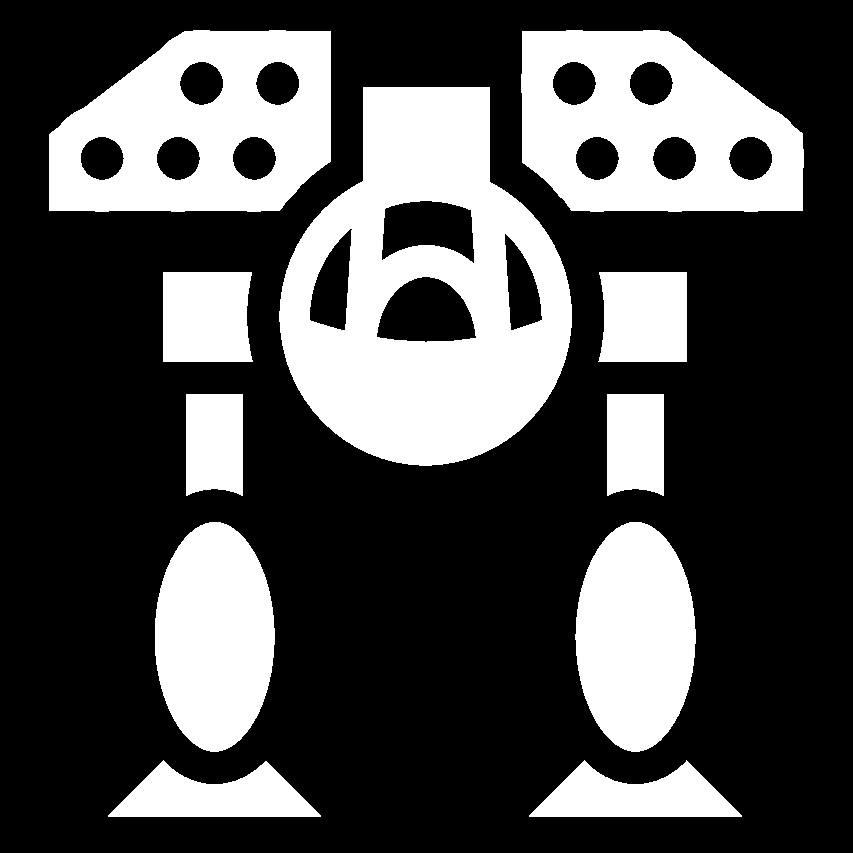
\includegraphics[width=3cm]{missile-mech}
  \caption{The insignia of 3rd Stompers}
  \label{fig:stompers}
\end{marginfigure}

\subsection{Officers}

\newthought{Commander of the 3rd Stompers} is Brigadier General \O yvind
Nordskov, who has rather traditional view on the role of his unit. On his
opinion, BattleMechs are the primary unit in battles and all other units are
there to support them. His views have caused clashes with other commanders
more than once. However, he is very skilled commander and can utilize
strengths of his unit very well.

\subsection{Tactics}

\newthought{Brigadier General Nordskov} prefers to take advantage of good
mobility of his 'mech forces and often circles around the opposing force in
order to attack their flank or rear with fast moving light and medium 'mechs.

\bigskip
\ovalbox{
\begin{minipage}{10cm}
15th Heavy Metal

BattleMech Regiment / Veteran / Reliable

CO: Colonel \`{A}sta Agnarsdottir

15th Heavy Metal is the hard hitting 'Mech unit that has been proved in battle
time and time again. The 15th Heavy Metal has very aggressive stance on
fighting and they mercilessly exploit any opening the opposing forces might
provide.
\end{minipage}}

\begin{marginfigure}[0\baselineskip]
  
\includegraphics[width=3cm]{cog}
  \caption{The insignia of 15th Heavy Metal}
  \label{fig:heavy_metal}
\end{marginfigure}

\bigskip
\ovalbox{
\begin{minipage}{10cm}
16th Hell Riders

BattleMech Regiment / Veteran / Reliable

CO: Colonel Erik Virtanen

16th Hell Riders have generally lighter 'Mechs that the 15th Heavy Metal, but
this doesn't mean they would shy away from the opposing force. The 16th Hell
Riders is often deployed on the flanks, where they harass opposing force with
their fast moving 'Mechs.
\end{minipage}}

\begin{marginfigure}[0\baselineskip]
  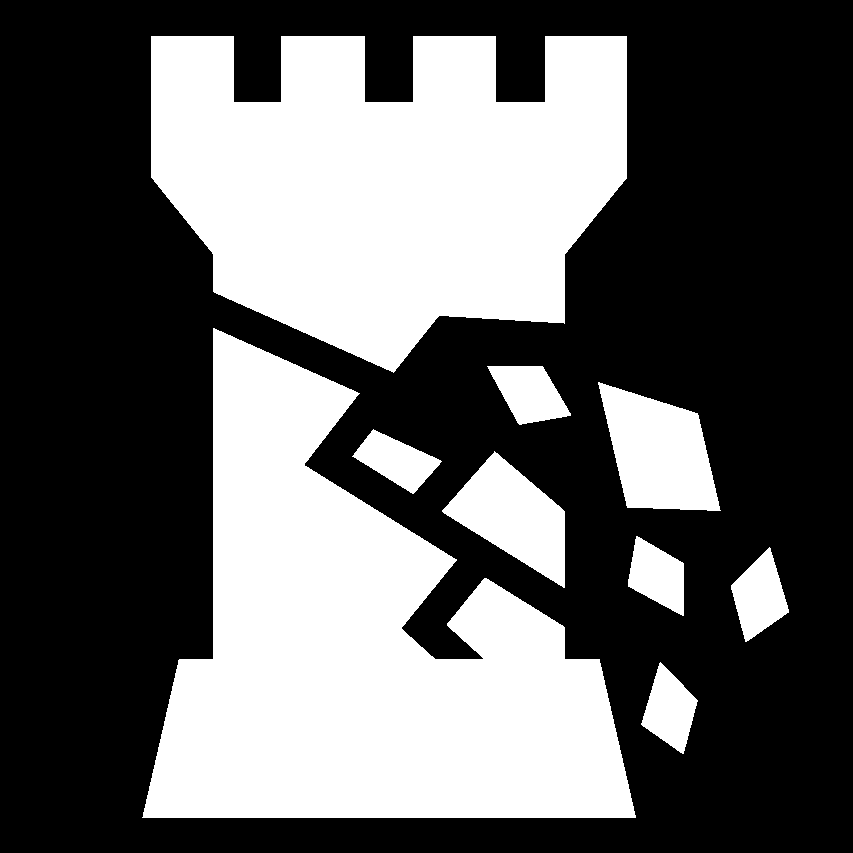
\includegraphics[width=3cm]{tower-fall}
  \caption{The insignia of 16th Hell Riders}
  \label{fig:hell_riders}
\end{marginfigure}

\bigskip
\ovalbox{
  \begin{minipage}{10cm}
    18th 'Mech Riders

    Mechanized Infantry Regiment / Veteran / Reliable

    CO: Colonel Jouni Olesen

    18th 'Mech Riders has long history with fighting alongside of 'Mech forces.
    Especially in urban environment they offer extra eyes on the ground and flush
    out ambushing enemies. In more open areas they usually follow behind the main
    force and clean up the opposing force units that 'Mechs missed.
\end{minipage}}

\begin{marginfigure}[0\baselineskip]
  
\includegraphics[width=3cm]{overdrive}
  \caption{The insignia of 18th Mech Riders}
  \label{fig:mech_riders}
\end{marginfigure}

\section{4th Winged Vengeance}

\newthought{4th Winged Vengeance} is the only active AeroSpace division in
KAF. They are tasked in patrolling and protecting Kiiminki system and
individual planets.

\begin{marginfigure}[0\baselineskip]
  
\includegraphics[width=3cm]{evil-wings}
  \caption{The insignia of 4th Winged Vengeance}
  \label{fig:winged_vengeance}
\end{marginfigure}

\subsection{Officers}

\newthought{Commander of the 4th Winged Vengeance} is Brigadier General
Ragnhei\dh ur Sigurdsdottir. In addition to arranging and coordinating the
AeroSpace defence of Kiiminki system, she is also tasked providing training
for fighter pilots of the merchant fleet.

\subsection{Tactics}

\newthought{4th Winged Vengeance} does not have enough AeroSpace fighters or
pilots to cover Kiiminki system sufficiently. Brigadier General Sigurdsdottir
works in close cooperation with intelligence branches and focuses the patrol
duties where they are the most effective. Due to material shortage, the 4th
Winged Vengeance carefully avoids any unnecessary risks and fights
conservatively.

\bigskip
\ovalbox{
  \begin{minipage}{10cm}
    20th Guardians

    2 AeroSpace Regiments / Elite / Reliable

    CO: Colonel Maarit Pajari

    XO: Colonel Ingrid Lager

    The 20th Guardians is nominally deployed in the Kiiminki Prime. They perform
    patrol flights on and around the planet. Heaviest AeroSpace fighters deployed
    by KAF are found in this unit.
\end{minipage}}

\begin{marginfigure}[0\baselineskip]
  
\includegraphics[width=3cm]{winged-sword}
  \caption{The insignia of 20th Guardians}
  \label{fig:guardians}
\end{marginfigure}

\bigskip
\ovalbox{
  \begin{minipage}{10cm}
    21st Protectors

    2 AeroSpace Regiments / Veteran / Reliable

    CO: Colonel Johan Alfsson

    XO: Colonel Hanna Solberg

    21st Protectors perform patrol flights deep in Kiiminki system. Thus their
    fighters tend to favour long range endurance and extensive sensor systems.
    They also perform escort missions for dropships when needed and often train
    together with the merchant fleet.
\end{minipage}}

\begin{marginfigure}[0\baselineskip]
  
\includegraphics[width=3cm]{steelwing-emblem}
  \caption{The insignia of 21st Protectors}
  \label{fig:protectors}
\end{marginfigure}

\bigskip
\ovalbox{
  \begin{minipage}{10cm}
    22nd Dusters

    2 AeroSpace Regiments / Regular / Reliable

    CO: Colonel Geir Haugen

    XO: Colonel Jukka Sel\"{a}nne

    22nd Dusters is nominally deployed in Jalanti, where they perform patrol
    flights. In addition to patrol duties, the 22nd Dusters trains new pilots.
    Their AeroSpace fighter selection is very broad, in order to give new pilots
    chance to train with different types of fighters.
\end{minipage}}

\begin{marginfigure}[0\baselineskip]
  
\includegraphics[width=3cm]{winged-emblem}
  \caption{The insignia of 22nd Dusters}
  \label{fig:dusters}
\end{marginfigure}

\chapter{Societies}
\label{ch:societies}

\newthought{Like any kingdom} Kiiminki has its share of secret and not so
secret societies. Some of these are mostly harmless, while others have more
nefarious purpose. Even within a single organisation there might be people
with differing agendas and methods.

\newthought{Kiiminki Peace Movement} is group of people concerned of
militarization of Kiiminki System. Their goal is to reduce military presence
in the system and eventually make Kingdom of Kiiminki a place without standing
army.

Majority of its members believe in non-violent demonstrations and affecting to
public opinion via leaflets, books and videos. There is small sub-group within
them, who have much more radical views and have an opinion that the end
justifies means. These radicals of Kiiminki Peace Movement are ready to hold
violent demonstrations and aggravate military forces to take action against
them in order to sway the public on their side.

Kiiminki Peace Movement started in 3015 and was founded by a small group of
students lead by Samuli Stigsson, who was a student of literature at the time.
Stigsson was killed in a demonstration turned into a riot in 3025, which
solidified his place in history as the martyr for the cause.

Current leader of the movement is Laura Naess, who has tried to guide the
movement back to its more peaceful roots. However, her attempts have not been
successful and the radical parts of the movement are growing. Her more
detailed bio can be found in section \ref{sc:laura-naess}

\newthought{Equatorial Liberation Army} is a rag-tag group who want to
separate equatorial regions of Kiiminki prime from rest of the kingdom of
Kiiminki and declare them to an independent nation. The group is very
disperse and doesn't have a firm leadership, structure or method of operation.

Military intelligence is keeping an eye on the known members and local police
forces intervene when the group activity is starting to cause problems or
damage.

There are rumours that the ELA has been negotiation with the pirate forces in
nearby systems and secured promise of supplies, training and man power to
their cause. Intelligence has not been able to confirm this, but is working
on the case.

\newthought{Friends of Nature} is group of people wanting to preserve nature
of Kiiminki Prime as much as possible. They would like to stop open-pit mining
and oil drilling. In addition to that, usage of internal combustion engines
should be limited and use fuel cells and fusion engines more than currently.

Friends of Nature are rather radical group, resorting in bomb attacks against
mines, drilling sites and refineries. Officially Friends of Nature is
classified as a criminal group and local police forces are actively trying to
apprehend members of it.

Rumours are that Kristian M\o ller is the leader of the organisation, but
concrete proofs are lacking and officials have not been able to arrest him.
M\o ller is actively advocating for sustainable way of living, but he
strictly denies all connections with the group. His complete bio is presented
in section \ref{sc:kristian-moller}.

\chapter{Notable People}
\label{ch:notable-people}

\newthought{Kingdom of Kiiminki} has many notable people and the available
space does not permit going through all of them. However, some highlights
can be shown in this section.

\subsection{Brigadier General Mari Lundgren}
\label{sc:bio-mari-lundgren}

\newthought{Brigadier general} Mari Lundgren is from a military family and
daughter of famous Major Mats Lundgren, commanded lead armored battalion during
operation Desert Fox. Brigadier general Lundgren started her military career
in xxx in 3033 at the age of 17. She volunteered to start her mandatory
military training a year earlier than what was usual.

Lundgren is the current commander of the
1st Arctic Strikers. She rose to the position in 3057, after being commander of
the 3rd Arctic Foxes for 5 years. In occasion, she has been accused of
favouring the 3rd Arctic Foxes over other units in the 1st Arctic Foxes.
However, these accusations are generally not supported by the members of her
unit.

Brigadier general Lundgren has been steadily introducing changes on how the
1st Arctic Strikers train and operate. It seems that she has ambitions to
change how KAF in general employs both regular and mechanized infantry in
combat. This is not possible in her current position, so it's expected that
she is trying to move into higher position and eventually be in charge of
KAF army branch.

\subsection{Peace Activist Laura Naess}
\label{sc:laura-naess}

\newthought{Laura Naess} is the 3rd child of a metal worker family. Both her
father and mother are employed by Wilkman Metal Works. Her father, Petter
Naess, works as a welder in a factory while her mother, Susann Naess, is a
power transmission designer.

In 3052 Laura enrolled into university to study global politics. While working
on her thesis on civilian treatment during Succession Wars, she came into
contact with the Kiiminki Peace Movement and soon joined it. After finishing
her studies in 3058, she started working in a local newspaper, while
maintaining contact with the peace movement.

In 3064, Laura was selected as a leader of the peace movement. She has been
trying to lead the movement back to its more peaceful ways and has partly
succeed. However, there still exists small, but vocal sub-group who believes
in direct action and aggravating the military to take action against them.

\subsection{Conservatist Kristian M\o ller}
\label{sc:kristian-moller}

Kristian was born.

\subsection{Metal Magnate Olof Wilkman}
\label{sc:bio-olof-wilkman}

\newthought{Olof Wilkman} was born too.

\subsection{Upstart Johann Wilkman}
\label{sc:bui.johann-wilkman}

\newthought{Johann Wilkman} is son of Olof Wilkman and expected to step up
and take over Olof's duties in Wilkman Metal Works.

\chapter{Life Modules}
\label{sc:life-modules}

\newthought{Life modules} are way to creating characters in A Time of War
roleplaying game. This section details some new modules that a character
hailing from Kingdom of Kiiminki may choose.

\bigskip
\begin{table}
\begin{minipage}{\textwidth}
\begin{center}
\begin{tabular}{ll}
\toprule
\multicolumn{2}{l}{Kingdom of Kiiminki} \\
Module cost: & 75 XP \\
\multirow{6}{*}[0.75em]{} & Kingdom of Kiiminki is situated in deep  \\
                          & periphery and has little contact with    \\
                          & the inner sphere. Some more adventurous  \\
                          & folk leave the planet to try their luck, \\
                          & while others find their calling in the   \\
                          & icy fields of Kiiminki Prime.            \\
Primary language: & Norwegian \\
Secondary languages: & Finnish, English \\
Fixed XPs: & \\
\quad Attributes & \\
& WIL (+60 XP) \\
\quad Traits & \\
& Equipped (-50 XP) \\
& Thick-Skinned (+25 XP) \\
\quad Skills & \\
& Interest/Any (+10 XP) \\
& MedTech/General (+15 XP) \\
& Small Arms (+15 XP) \\
& Survival/Arctic (+50 XP) \\

\multirow{3}{*}[0.75em]{Flexible XPs:} \\
                                       & +10 XP each to any two Attributes, Traits \\
                                       & or Skills or combination thereof \\

\bottomrule
\end{tabular}
\end{center}
\end{minipage}
\caption{Affliation: Kingdom of Kiiminki}
\end{table}

\bigskip
\begin{table}
\begin{minipage}{\textwidth}
\begin{center}
\begin{tabular}{ll}
\toprule
\multicolumn{2}{l}{Arctic Explorer} \\

\multirow{6}{*}[0.75em]{} & Arctic explorers roam in the deep arctic \\
                          & of Kiiminki Prime, mapping and exploring \\
                          & the area in detail. They are masters in  \\
                          & arctic survival and often even employed  \\
                          & by KAF as path finders and guides in the \\
                          & icy polar areas.                         \\


Module cost: & 900 XP \\
Prerequisites: & Cannot have thin-skinned trait \\
Time: & +6 years \\
Fixed XPs: & \\
\quad Attributes & \\
& BOD (+40 XP) \\
& INT (+30 XP) \\
& WIL (+30 XP) \\
\quad Traits & \\
& Good Vision (+50 XP) \\
& Patient (+50 XP) \\
& Thick-Skinned (+50 XP) \\
\quad Skills & \\
& Climbing (+70 XP) \\
& Communications/Conventional (+70 XP) \\
& Driving/Ground (+50 XP) \\
& MedTech/General (+50 XP) \\
& Navigation/Land (+70 XP) \\
& Perception (+50 XP) \\
& Sensor Operations (+50 XP) \\
& Survival/Arctic (+70 XP) \\
Flexiple XPs: & +170 XP \\

\bottomrule
\end{tabular}
\end{center}
\end{minipage}
\caption{Real Life: Arctic Explorer}
\end{table}


\chapter{Support Vehicles}
\label{ch:support-vehicles}


\newthought{Support vehicles} form an essential part of any planet's
backbone. They might not be as flashy as machines of war, but without
them a planet would be in trouble.

This section will detail some new support vehicles that have been
designed specifically to work in the arctic environment.



\section{Snow Mover}
\newthought{Snow Mover} is a cheap and simple truck aimed for snow clearing and
removal. Two man crew is needed to effectively manage clearing equipment
and large searchlights mounted on the roof of the truck.

Snow Mover is the first dedicated snow clearing equipment by Drago ltd. As
such, it was based on very primitive technology as the goal was to build
cheap, sturdy and easy to maintain vehicle.

The vehicle didn't gain very widespread adoption. Partly because the very
specialized niche and partly because it was pretty terrible in clearing
snow. Wheeled design tended to get stuck in snow and it suffered from
other malfunctions too\marginnote{The engine was notoriously slow to accelerate 
  and would use disproportionate amounts of gas when driven at full speed.
  On top of that, Snow Mover lacks even the most basic armour, making it
  vulnerable to accidents.}.

\bigskip
\begin{table}
  \begin{minipage}{\textwidth}
    \begin{center}
      \begin{tabular}{llll}
        \toprule
        Type: & Snow Mover & \\
        Chassis Type: & Wheeled (Medium) & \\
        Mass: & 10 tons & \\
        Tech base: & Inner Sphere & \\
        Equipment Rating: & C-C-C & \\
        Availability: & X-B-B & \\
        Production Year: & 3025 & \\
        Cost: & 88 200? & \\
        Battle Value: & & \\
        Manufacturer: & Drago, Ltd & \\
        Equipment & & Mass \\
        \quad Chassis/Controls: & & 2.0 \\
        \quad Engine/Trans: & ICE  & 3.0 \\
        \quad Fuel: & 1660 km (Petrochemical) & 0.5 \\
        \quad Speed: & \multicolumn{2}{l}{4/6} \\
        Structure and Armour & & \\
        \quad Armor Factor (N/A): & N/A & N/A \\
        \quad & Internal & Armor \\
        \quad Front & 1 & 0 \\
        \quad R/L Side & 1 & 0 \\
        \quad Rear & 1 & 0 \\
        Armament and Capabilities: & & \\
        \multicolumn{2}{l}{\quad Bulldozer, Front} & 2.0 \\
        \multicolumn{2}{l}{\quad Dumper, backfacing} & 50kg \\
        \multicolumn{2}{l}{\quad 2 Search lights, Front and Back} & 0.5 each \\

        \multicolumn{3}{l}{Crew: 2} \\
        Cargo: & & \\
        \multicolumn{3}{l}{\quad 1 ton bulk (1 ton), with a dumper} \\

        Notes: & & \\
        \multicolumn{3}{l}{\quad Easy to Maintain, Gas Hog, Poor Performance} \\
        \bottomrule
      \end{tabular}
    \end{center}
  \end{minipage}
  \caption{Snow Mover}
\end{table}


\section{Tracked Snow Mover}
\newthought{Not satisfied} with the original Snow Mover, Drago Ltd set to
design an improved version. The new version used tracks and was specifically
designed for snow operations. Using the easy to maintain diesel power
plant meant that the vehicle was slower than before, with a top speed
of 54 km/h\marginnote{Originally engineers wanted to have the vehicle to have
  a top speed of 64.8 km/h, but that simply wasn't possible with the chosen
  engine type.} and was burning through fuel at a high rate when driven at top
speed.

Tracked snow mover was fitted with half a ton of BAR 4 armour, that would
protect it against accidental glances and falling debris. While not
originally designed to work as a bulldozer, tracked snow mover could be used
in such an operation too.

\bigskip
\begin{table}
  \begin{minipage}{\textwidth}
    \begin{center}
      \begin{tabular}{llll}
        \toprule
        Type: & Tracked Snow Mover & \\
        Chassis Type: & Tracked (Medium) & \\
        Mass: & 25 tons & \\
        Tech base: & Inner Sphere & \\
        Equipment Rating: & C-C-C & \\
        Availability: & X-B-B & \\
        Production Year: & 3030 & \\
        Cost: & 228 625 & \\
        Battle Value: & & \\
        Manufacturer: & Drago, Ltd & \\
        Equipment & & Mass \\
        \quad Chassis/Controls: & & 8.0 \\
        \quad Engine/Trans: & ICE & 8.0 \\
        \quad Fuel: & 625 km (Petrochemical) & 0.5 \\
        \quad Speed: & \multicolumn{2}{l}{3/5} \\
        Structure and Armour & & \\
        \quad Armor Factor (BAR 4): & 31 & 1.0 \\
        \quad & Internal & Armor \\
        \quad Front & 3 & 10 \\
        \quad R/L Side & 3 & 7 \\
        \quad Rear & 3 & 7 \\

        Armament and Capabilities: & & \\
        \multicolumn{2}{l}{\quad Bulldozer, Front} & 2.0 \\
        \multicolumn{2}{l}{\quad Dumper, backfacing} & 50kg \\
        \multicolumn{2}{l}{\quad Search light, Front} & 0.5 \\

        \multicolumn{3}{l}{Crew: 2} \\
        Cargo: & & \\
        \multicolumn{3}{l}{\quad 1 ton bulk (1 ton), with a dumper} \\

        Notes: & & \\
        \multicolumn{3}{l}{\quad Snowmobile, Easy to Maintain, Gas Hog} \\

        \bottomrule
      \end{tabular}
    \end{center}
  \end{minipage}
  \caption{Tracked Snow Mover}
\end{table}



\chapter{Combat Vehicles}
\label{ch:combat-vehicles}


\newthought{Combat vehicles} are the bread and butter of any army.

This section will detail some new combat vehicles that have been
designed specifically to work in the arctic environment.


\section{Snow Leopard SLP-1}

\newthought{Heavily armoured} Snow Leopard is first completely new design
by Wilkman Metal Works utilizing fusion engine. It was contracted by the KAF,
who wanted a medium weight tank with high survivability and decent fire power.

Snow Leopard was designed as main battle tank for the 2nd Raiders, who helped
Wilkman Metal Works to run the trials and fine tune the design. One of their
requests was that the main weapon would be ammo-independent, which lead to
PPC.

SLP-1 one complicated and expensive to manufacture and the 2nd Raiders have
only received small number of them so far.

\bigskip
\begin{table}
\begin{minipage}{\textwidth}
\begin{center}
\begin{tabular}{llll}
\toprule
Type: & Snow Leopard SLP-1 & \\
Chassis Type: & Tracked (Medium) & \\
Mass: & 50 tons & \\
Tech base: & Inner Sphere & \\
Rating: & D/X-E-D & \\
Production Year: & 3025 & \\
Cost: & 1 967 500 & \\
Battle Value: & 959 & \\
Manufacturer: & Wilkman Metal Works & \\
Equipment & & Mass \\
\quad Chassis/Controls: & & 7.5 \\
\quad Engine/Trans: & Fusion & 13.0 \\
\quad Fuel: & - & - \\
\quad Speed: & \multicolumn{2}{l}{4/6} \\
Structure and Armour & & \\
\quad Armor Factor: & 208 & 13.0 \\
\quad & Internal & Armor \\
\quad Front & 5 & 52 \\
\quad R/L Side & 5 & 41 \\
\quad Rear & 5 & 34 \\
\quad Turret & 5 & 40 \\

Armament and Capabilities: & & \\
\multicolumn{2}{l}{\quad LRM-10, Front} & 5.0 \\
\multicolumn{2}{l}{\quad PPC, Turret} & 7.0 \\
\multicolumn{2}{l}{\quad LRM-10 Ammunition} & 2.0 \\
\multicolumn{2}{l}{\quad Machine Gun Ammunition} & 1.0 \\


\multicolumn{3}{l}{Crew: 4} \\

Notes: & & \\


\bottomrule
\end{tabular}
\end{center}
\end{minipage}
\caption{Snow Leopard SLP-1}
\end{table}


\section{Snow Leopard SLP-2}

\newthought{While SLP-2} was popular design, it was difficult and expensive to
manufacture. Wilkman Metal Works designed a cheaper and less complex version
of the vehicle, that used internal combustion engine instead of the fusion
engine. As a result, the top speed dropped somewhat and weaponry needed to be
scaled down.

SLP-2 is currently being used where SLP-1 couldn't be delivered yet. Slower
top speed makes design better suited to statical defense instead of dynamic
attack.

\bigskip
\begin{table}
\begin{minipage}{\textwidth}
\begin{center}
\begin{tabular}{llll}
\toprule
Type: & Snow Leopard SLP-2 & \\
Chassis Type: & Tracked (Medium) & \\
Mass: & 50 tons & \\
Tech base: & Inner Sphere & \\
Rating: & D/X-D-C & \\
Production Year: & 3025 & \\
Cost: & 955 500 & \\
Battle Value: & 775 & \\
Manufacturer: & Wilkman Metal Works & \\
Equipment & & Mass \\
\quad Chassis/Controls: & & 7.5 \\
\quad Engine/Trans: & I.C.E. & 11.0 \\
\quad Fuel: & 600 km & - \\
\quad Speed: & \multicolumn{2}{l}{3/5} \\
Structure and Armour & & \\
\quad Armor Factor: & 200 & 12.5 \\
\quad & Internal & Armor \\
\quad Front & 5 & 48 \\
\quad R/L Side & 5 & 40 \\
\quad Rear & 5 & 32 \\
\quad Turret & 5 & 40 \\

Armament and Capabilities: & & \\
\multicolumn{2}{l}{\quad Large Laser, Turret} & 5.0 \\
\multicolumn{2}{l}{\quad Medium Laser, Turret} & 1.0 \\
\multicolumn{2}{l}{\quad Power Amplifiers} & 1.0 \\

\multicolumn{3}{l}{Crew: 4} \\

Notes: & & \\


\bottomrule
\end{tabular}
\end{center}
\end{minipage}
\caption{Snow Leopard SLP-2}
\end{table}


\section{Snow Ferret SNF-1}

\newthought{KFA contracted} Wilkman Metal Works to design and manufacture a
new recon armor to complement the new Snow Leopard. The result was Snow
Ferret, 40 ton, lightly armoured and armed recon armor.

SNF-1 model uses fusion engine, making it difficult and expensive to
manufacture, but the KAF armor commanders are quite pleased with the
combination of speed, protection and firepower of the vehice.

\bigskip
\begin{table}
\begin{minipage}{\textwidth}
\begin{center}
\begin{tabular}{llll}
\toprule
Type: & Snow Ferret SNF-1 & \\
Chassis Type: & Tracked (Medium) & \\
Mass: & 40 tons & \\
Tech base: & Inner Sphere & \\
Rating: & D/X-D-D & \\
Production Year: & 3025 & \\
Cost: & 1 128 167 & \\
Battle Value: & 435 & \\
Manufacturer: & Wilkman Metal Works & \\
Equipment & & Mass \\
\quad Chassis/Controls: & & 6.0 \\
\quad Engine/Trans: & Fusion & 13.0 \\
\quad Fuel: & - & - \\
\quad Speed: & \multicolumn{2}{l}{5/8} \\
Structure and Armour & & \\
\quad Armor Factor: & 88 & 5.5 \\
\quad & Internal & Armor \\
\quad Front & 4 & 22 \\
\quad R/L Side & 4 & 17 \\
\quad Rear & 4 & 18 \\
\quad Turret & 4 & 18 \\

Armament and Capabilities: & & \\
\multicolumn{2}{l}{\quad 2 Autocannon/2, Turret} & 12.0 \\
\multicolumn{2}{l}{\quad Autocannon/2 Ammunition} & 2.0 \\


\multicolumn{3}{l}{Crew: 3} \\

Notes: & & \\


\bottomrule
\end{tabular}
\end{center}
\end{minipage}
\caption{Snow Ferret SNF-1}
\end{table}


\section{Protector PTR-1}

\newthought{The very latest prototype} Protector PTR-1 utilizes new cluster
technology for autocannons, making it very effective against airborne targets.
The drawback is that autocannons have to be imported and they are hard to
obtain.

There are only few prototypes of Protector PTR-1 in existence. All have been
assigned to the 11th Fly Swatters for field trials. It will be several years
still until it will enter into more widespread usage, if the field trials deem
the design suitable.

\bigskip
\begin{table}
\begin{minipage}{\textwidth}
\begin{center}
\begin{tabular}{llll}
\toprule
Type: & Protector PTR-1 & \\
Chassis Type: & Tracked (Heavy) & \\
Mass: & 60 tons & \\
Tech base: & Inner Sphere & \\
Rating: & E/X-X-E & \\
Production Year: & 3068 & \\
Cost: & 2 484 000 & \\
Battle Value: & 813 & \\
Manufacturer: & Wilkman Metal Works & \\
Equipment & & Mass \\
\quad Chassis/Controls: & & 9.0 \\
\quad Engine/Trans: & Fusion & 10.5 \\
\quad Fuel: & - & - \\
\quad Speed: & \multicolumn{2}{l}{3/5} \\
Structure and Armour & & \\
\quad Armor Factor: & 208 & 13.0 \\
\quad & Internal & Armor \\
\quad Front & 6 & 51 \\
\quad R/L Side & 6 & 41 \\
\quad Rear & 6 & 33 \\
\quad Turret & 6 & 42 \\

Armament and Capabilities: & & \\
\multicolumn{2}{l}{\quad 4 LB 2-X Autocannon, Turret} & 24.0 \\
\multicolumn{2}{l}{\quad LB 2-X Autocannon Ammunition} & 1.0 \\


\multicolumn{3}{l}{Crew: 4} \\

Notes: & & \\


\bottomrule
\end{tabular}
\end{center}
\end{minipage}
\caption{Protector PTR-1}
\end{table}


\chapter{IndustrialMechs}
\label{ch:industrialmechs}


\newthought{IndustrialMechs} are much more versatile than support vehicles
when it comes to traveling on a difficult terrain. They are also quite
a bit more expensive and harder to maintain.

This section will detail some new IndustrialMechs that have been
designed specifically to work in the arctic environment.


\section{Digger DGR-1A}
\newthought{Digger} was designed as a mining 'mech, with specific focus
on breaking stone and loading it onto other 'mech or vehicle. It does not
have any cargo capacity, but sports rock cutter and backhoe.

\marginnote[+7cm]{While fusion engine has cheap running costs and long range,
maintenance is a lot more difficult than more conventional engines require.
Not all customers were happy about the decision to use it.}
\marginnote[+1.8cm]{DGR-1A uses standard armour, which protects it well against
rigours of mining work.}

\bigskip
\begin{table}
\begin{minipage}{\textwidth}
\begin{center}
\begin{tabular}{llll}
\toprule
Type: & Digger DGR-1A & \\
Chassis Type: & Biped Industrial & \\
Mass: & 25 tons & \\
Tech base: & Inner Sphere & \\
Rating \& Availability: & D/D-D-A & \\
Production Year: & 3025 & \\
Cost: & 984 052 & \\
Battle Value: & 213 & \\
Manufacturer: & ? & \\
Equipment & & Mass \\
\quad Chassis/Controls: & Industrial & 5.0 \\
\quad Armor Factor: & Standard & 2.5 \\
\quad Engine/Trans: & Fusion Engine & 3.0 \\
\quad Fuel: & ? & ? \\
\quad Speed: & \multicolumn{2}{l}{4/6/0} \\
\quad Heatsinks: & Single Heat Sink & 0.0 \\
\quad Heatsink locations: & 2 CT, 2 LL, 2 RL & \\
\quad Gyro: & Standard & 1.0 \\
\quad Cockpit: & Industrial & 3.0 \\
\quad Actuators: & Left: SH+UA+LA & Right: SH+UA+LA \\
Structure and Armour & Internal & Armor \\
\quad Head & 3 & 7 \\
\quad Center Torso & 8 & 6 \\
\quad Center Torso (rear) & - & 1 \\
\quad L/R Torso & 6 & 5 \\
\quad L/R Torso (rear) & - & 1 \\
\quad L/R Arm & 4 & 3 \\
\quad L/R Leg & 6 & 4 \\

Armament and Capabilities: & & \\
\quad Searchlight & Head & 0.5 \\
\quad Rock cutter & Right Arm & 5.0 \\
\quad Backhoe & Left Arm & 5.0 \\

Notes: & & \\
\multicolumn{3}{l}{\quad } \\

\bottomrule
\end{tabular}
\end{center}
\end{minipage}
\caption{Digger DGR-1A}
\end{table}

\section{Digger DGR-1D}
\newthought{Digger 1D} is a I.C.E. version of the earlier A-model. 
I.C.E. and commercial armour are quite a bit cheaper and there
is no too big drop in the performance. As a result D-model is 
very popular one, especially in the operations that have very limited 
resource pool.

\marginnote[+7cm]{Performance of I.C.E. engine may not be as good as
fusion engine's, but the cost is signigically lower. The problem is that
fuel consumption is far more greater.}
\marginnote[+2cm]{Commercial armour doesn't protect as well as the
standard one, but it is usually more than enough for a mining 'mech.}

\bigskip
\begin{table}
\begin{minipage}{\textwidth}
\begin{center}
\begin{tabular}{llll}
\toprule
Type: & Digger DGR-1D & \\
Chassis Type: & Biped Industrial & \\
Mass: & 25 tons & \\
Tech base: & Inner Sphere & \\
Rating \& Availability: & D/D-D-A & \\
Production Year: & 3025 & \\
Cost: & 818 391 & \\
Battle Value: & 143 & \\
Manufacturer: & ? & \\
Equipment & & Mass \\
\quad Chassis/Controls: & Industrial & 5.0 \\
\quad Armor Factor: & Commercial & 1.5 \\
\quad Engine/Trans: & I.C.E. & 4.0 \\
\quad Fuel: & 600 km & 0.0 \\
\quad Speed: & \multicolumn{2}{l}{3/5/0} \\
\quad Heatsinks: & Single Heat Sink & 0.0 \\
\quad Heatsink locations: &  & \\
\quad Gyro: & Standard & 1.0 \\
\quad Cockpit: & Industrial & 3.0 \\
\quad Actuators: & Left: SH+UA+LA & Right: SH+UA+LA \\
Structure and Armour & Internal & Armor \\
\quad Head & 3 & 6 \\
\quad Center Torso & 8 & 5 \\
\quad Center Torso (rear) & - & 1 \\
\quad L/R Torso & 6 & 4 \\
\quad L/R Torso (rear) & - & 1 \\
\quad L/R Arm & 4 & 3 \\
\quad L/R Leg & 6 & 4 \\

Armament and Capabilities: & & \\
\quad Searchlight & Head & 0.5 \\
\quad Rock cutter & Right Arm & 5.0 \\
\quad Backhoe & Left Arm & 5.0 \\

Notes: & & \\
\multicolumn{3}{l}{\quad } \\

\bottomrule
\end{tabular}
\end{center}
\end{minipage}
\caption{Digger DGR-1D}
\end{table}



\section{Digger DGR-1F}
\newthought{Digger 1F} is a fuel-cell variant of the earlier A-model.
Performance is on par with the DGR-1A in all other areas
execpt on operation range and armour. Fuel-cell model was never really
popular since operations with cash to spare generally selected fusion
engine one, while others opted for I.C.E.

\marginnote[+7cm]{Fuel-Cell engine is only slightly heavier than
the fusion one and the performance is pretty much equal.}

\bigskip
\begin{table}
\begin{minipage}{\textwidth}
\begin{center}
\begin{tabular}{llll}
\toprule
Type: & Digger DGR-1F & \\
Chassis Type: & Biped Industrial & \\
Mass: & 25 tons & \\
Tech base: & Inner Sphere & \\
Rating \& Availability: & D/D-D-A & \\
Production Year: & 3025 & \\
Cost: & 911 271 & \\
Battle Value: & 147 & \\
Manufacturer: & ? & \\
Equipment & & Mass \\
\quad Chassis/Controls: & Industrial & 5.0 \\
\quad Armor Factor: & Commercial & 1.5 \\
\quad Engine/Trans: & Fuel-Cell & 4.0 \\
\quad Fuel: & 450 km & 0.0 \\
\quad Speed: & \multicolumn{2}{l}{4/6/0} \\
\quad Heatsinks: & Single Heat Sink & 0.0 \\
\quad Heatsink locations: &  & \\
\quad Gyro: & Standard & 1.0 \\
\quad Cockpit: & Industrial & 3.0 \\
\quad Actuators: & Left: SH+UA+LA & Right: SH+UA+LA \\
Structure and Armour & Internal & Armor \\
\quad Head & 3 & 6 \\
\quad Center Torso & 8 & 5 \\
\quad Center Torso (rear) & - & 1 \\
\quad L/R Torso & 6 & 4 \\
\quad L/R Torso (rear) & - & 1 \\
\quad L/R Arm & 4 & 3 \\
\quad L/R Leg & 6 & 4 \\

Armament and Capabilities: & & \\
\quad Searchlight & Head & 0.5 \\
\quad Rock cutter & Right Arm & 5.0 \\
\quad Backhoe & Left Arm & 5.0 \\

Notes: & & \\
\multicolumn{3}{l}{\quad } \\

\bottomrule
\end{tabular}
\end{center}
\end{minipage}
\caption{Digger DGR-1F}
\end{table}

\chapter{BattleMechs}
\label{ch:battlemechs}


\newthought{BattleMechs} are kings of the battle ground. 

This section will detail some new BattleMechs that have been
designed specifically to work in the arctic environment.

\clearpage

%%
% The back matter contains appendices, bibliographies, indices, glossaries, etc.







\backmatter

% \bibliography{sample-handout}
% \bibliographystyle{plainnat}


\printindex

\end{document}

